\subsection{Convertidor CC-CC Conmutado}

Para llevar a cabo el diseño del convertidor, primero debemos establecer los objetivos de rendimiento del mismo (como por ejemplo, la tensión que debe tener a la salida). Con estos valores establecidos, y junto con otras consideraciones del diseño, se van a obtener todos los parámetros que definen al convertidor, como las llaves y diodos a utilizar, tamaño de capacitores e inductores, etc.\\

\begin{figure}[h]
    \centering
    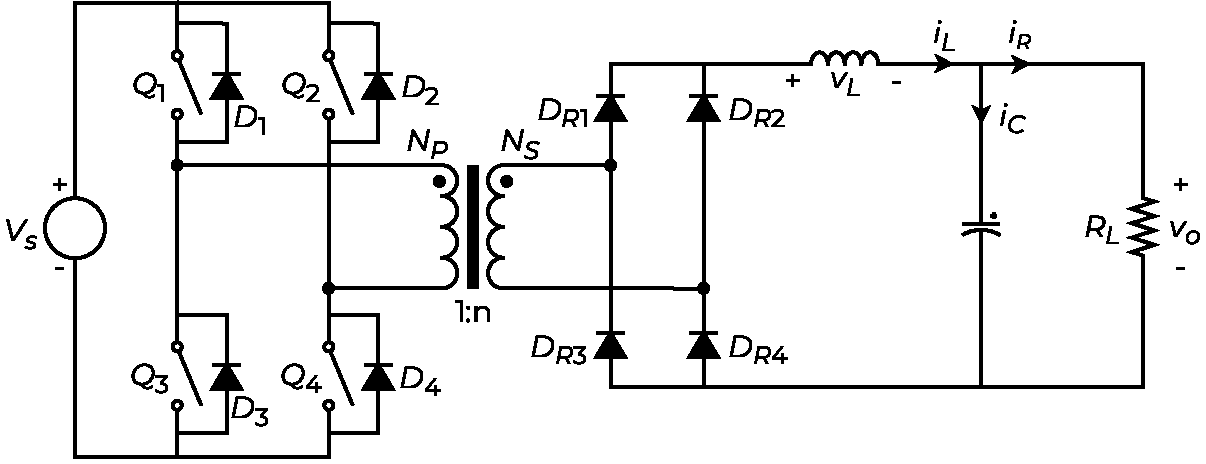
\includegraphics[scale=0.6]{Imagenes/Full Bridge.pdf}
    \caption{Diagrama del convertidor CC-CC de tipo puente completo a utilizar, con todos sus componentes.}
    \label{puente_completo}
\end{figure}

\subsubsection{Especificaciones de Diseño}

La plataforma experimental va a ser utilizada para la evaluación de un módulo de pilas de combustible de \SI[]{300}[]{\watt} de potencia nominal, entregando \SI[]{36}[]{\volt} a \SI[]{8.3}[]{\ampere} de corriente. La tensión de salida varía desde \SI[]{65}[]{\volt} a circuito abierto hasta \SI[]{30}[]{\volt} para la máxima corriente de \SI[]{9.5}[]{\ampere}.\textsuperscript{\cite{HSeriesBrochure}}\\

Esta potencia debe ser transferida por el convertidor hacia la carga variable a la salida, que emula distintas condiciones de carga del bus común de corriente continua de \SI[]{75}[]{\volt} fijos. Dada la potencia de \SI[]{300}[]{\watt}, y si la tensión de salida es la del bus común, entonces el sistema debe soportar una corriente de salida máxima de alrededor de \SI[]{4}[]{\ampere}. Adicionalmente, las llaves del primario van a conmutar a una frecuencia de conmutación de \SI[]{20}[]{\kilo\hertz}, y se debe reducir lo más posible las pérdidas de energía por conmutación, para darle una mayor escalabilidad al diseño.\\

\begin{itemize}
    \item {\SemiBold Potencia nominal \textit{P\textsubscript{N}}:}\quad\SI[]{300}[]{\watt}
    \item {\SemiBold Tensión de salida \textit{v\textsubscript{o}}:}\quad\SI[]{75}[]{\volt}
    \item {\SemiBold Corriente de salida \textit{i\textsubscript{o}}:}\quad\SI[]{4}[]{\ampere}
    \item {\SemiBold Tensión de entrada \textit{v\textsubscript{FC}}:}\quad\SI[]{45}[]{\volt}\textsubscript{máx} , \SI[]{28}[]{\volt}\textsubscript{mín}
    \item {\SemiBold Corriente de entrada \textit{i\textsubscript{FC}}:}\quad\SI[]{9.5}[]{\ampere}
    \item {\SemiBold Frecuencia de conmutación \textit{f\textsubscript{s}}:}\quad\SI[]{20}[]{\kilo\hertz}\\
\end{itemize}

Entonces, con todas estas características quedan definidas las especificaciones necesarias para comenzar la selección y dimensionamiento de componentes del convertidor. Se va a tratar el diseño de cada componente uno por uno, comenzando por los cuatro transistores de potencia que se encargan de la conmutación.\\

\subsubsection{Selección de Llaves}

Las cuatro llaves ideales que conforman el circuito puente del lado primario son implementadas por algún dispositivo electrónico de tres terminales (los dos terminales de potencia, y un tercer terminal de control con el que se comanda la conmutación de la llave). Existen dentro de estas llaves dos categorías distintas: las \textit{llaves semicontroladas}, donde la llave no se puede controlar completamente (por ejemplo se puede comandar el cierre pero no la apertura) y las \textit{llaves completamente controladas} que, como su nombre dice, pueden ser cerradas y abiertas mediante su tercer terminal.\\

En nuestro caso, la topología de puente completo exige la apertura y cierre de las cuatro llaves a la frecuencia de conmutación, por lo que se requieren {\Medium llaves completamente controladas}, dentro de las cuales se pueden elegir una serie de transistores o tiristores.\\

\paragraph{Tecnologías de Transistores}

En nuestro caso, nos vamos a enfocar únicamente en los tres tipos distintos de transistores de potencia, evaluandolos para su uso en la plataforma: el transistor bipolar o BJT (\textit{Bipolar Junction Transistor}), el transistor IGBT (\textit{Insulated-Gate Bipolar Transistor}) y el transistor de efecto de campo o MOSFET (\textit{Metal-Oxide-Semiconductor Field-Effect Transistor}).\\

\subparagraph{Transistor Bipolar}

El transistor bipolar de la figura \ref{bjt} cuenta con su terminal de control, la \textit{base} (B), y sus dos terminales de potencia, el \textit{colector} (C) y \textit{emisor} (E). Este dispositivo se controla mediante la inyección de corriente por la base, por lo que se puede decir que es una llave controlada por corriente.\\

\begin{figure}[h]
    \centering
    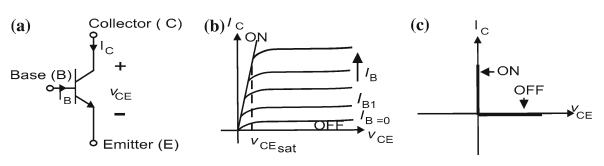
\includegraphics[scale=0.6]{Imagenes/BJT.png}
    \caption{El transistor bipolar (a) su símbolo eléctrico, (b) su curva característica, (c) su curva como llave ideal.}
    \label{bjt}
\end{figure}

Su funcionamiento viene dado por las curvas de corriente de colector $I_C$ contra tensión colector-emisor $V_{CE}$ en el primer cuadrante. El transistor se encuentra en su estado apagado (región de corte) en el área debajo de la curva de corriente de base $I_B$ nula; mientras que se encuentra encendido (región de saturación) en el área donde la tensión $V_{CE}$ es menor a la tensión de saturación ($V_{CE} \leq {V_{CE}}_{sat}$).\\

Hoy en día, los BJT rara vez son utilizados como llaves de potencia, ya que las otras dos tecnologías tienen grandes ventajas frente a este tipo de dispositivo. Primero, al ser un dispositivo controlado por corriente, estos transistores pierden mucha energía de forma disipativa al ser conmutados. Además, al ser un dispositivo de portadores minoritarios, su tiempo de conmutación se ve afectado, cayendo en el orden de los \unit[]{\micro\second}. Sin embargo, como ventaja tienen su baja impedancia de salida, lo que les da una muy baja pérdida de conducción.\textsuperscript{\cite{PotenciaHart}\cite{PowerElecRenewableEnergySystems}}\\

\subparagraph{MOSFET}

El MOSFET de la figura \ref{mosfet} tiene al \textit{gate} (G) como terminal de control, y los terminales de \textit{drain} (D) y \textit{source} (S) como terminales de potencia. Este transistor se controla mediante la variación de la tensión gate-source $V_{GS}$, por lo que, a diferencia del BJT, es un dispositivo controlado por tensión.\\

\begin{figure}[h]
    \centering
    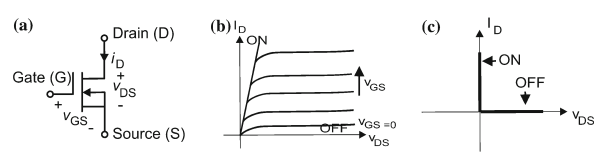
\includegraphics[scale=0.6]{Imagenes/MOSFET.png}
    \caption{El MOSFET (a) su símbolo eléctrico, (b) su curva característica, (c) su curva como llave ideal.}
    \label{mosfet}
\end{figure}

Su funcionamiento es caracterizado por las curvas de corriente de drain $I_D$ versus tensión drain-source $V_{DS}$ en el primer cuadrante. Para encontrarse en estado apagado o región de corte, la tensión de control $V_{GS}$ debe ser menor a una tensión umbral o \textit{threshold} $v_T$ que depende del dispositivo (esto corresponde a la región debajo de la marca OFF en la figura). Cuando la tensión de control supera este umbral, el dispostivo entra en conducción, con una resistencia drain-source ${R_{DS}}_{on}$ baja de orden de \unit[]{\milli\ohm}.\\

Los MOSFET tienen varias características que los hacen deseables como interruptores electrónicos de potencia: al ser controlados por tensión, la pérdida disipativa de potencia para la conmutación es muy baja; como el dispositivo trabaja con portadores mayoritarios, su velocidad de conmutación es muy rápida, con tiempos de conmutación en el orden de los \unit[]{\nano\second}; y tienen una alta impedancia de entrada. Además, por su construcción, tienen un diodo antiparalelo incluido entre D y S, cosa que es deseable para muchas topologías de convertidores.\\

Sin embargo, tienen como desventaja una limitación en tensión y corriente, ya que no soportan corrientes que excedan los \SI[]{200}[]{\ampere} ni tensiones por encima de \SI[]{1}[]{\kilo\volt}; además de tener una elevada impedancia de salida, generando pérdidas de conducción.\textsuperscript{\cite{PotenciaHart}\cite{PowerElecRenewableEnergySystems}}\\

\subparagraph{IGBT}

Los transistores del tipo IGBT podrían ser considerados como un híbrido entre las dos tecnologías anteriores, combinando las ventajas de ambos. Este dispositivo tiene un terminal de control llamado gate (G) al igual que el MOSFET, y dos terminales de potencia, el colector (C) y emisor (E), al igual que el BJT. Se controla mediante la tensión gate-emisor $V_{GE}$, por lo que es controlado por tensión al igual que el MOSFET.\\

\begin{figure}[h]
    \centering
    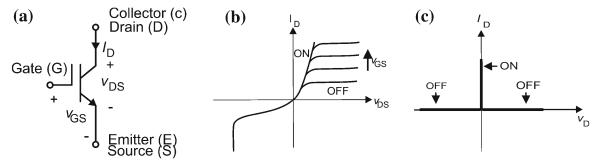
\includegraphics[scale=0.6]{Imagenes/IGBT.png}
    \caption{El IGBT (a) su símbolo eléctrico, (b) su curva característica, (c) su curva como llave ideal.}
    \label{igbt}
\end{figure}

Se caracteriza por la curva de corriente de colector $I_C$ contra tensión gate-emisor $V_{GE}$ de la figura \ref{igbt}, y a diferencia de los anteriores dos transistores, opera en los cuadrantes primero y segundo, es decir que puede bloquear tensión bidireccionalmente y conducir corriente de forma unidireccional.\\

Este transistor combina las ventajas de los BJT y los MOSFET, es decir que tiene una alta impedancia de entrada como el MOSFET, disminuyendo las pérdidas disipativas de la conmutación; una baja impedancia de salida como el BJT, disminuyendo las pérdidas de conducción; y soporta muy altas tensiones, por encima de \SI[]{1}[]{\kilo\volt}, y corrientes mayores a \SI[]{500}[]{\ampere}. Sin embargo, si bien su velocidad de conmutación es superior a la del transistor bipolar, pero no alcanza los cortos tiempos del orden de \unit[]{\nano\second} de los MOSFET, además de ser la tecnología más costosa dentro de las presentadas.\textsuperscript{\cite{PotenciaHart}\cite{PowerElecRenewableEnergySystems}}\\

\paragraph{Selección de MOSFET}

Como las llaves de la plataforma de evaluación nunca excederán los \SI[]{15}[]{\ampere}, y la tensión sobre las llaves no puede superar los \SI[]{70}[]{\volt}, los transistores del tipo MOSFET son la elección más lógica. Sus límites de tensión y corriente están muy por encima de los requierimientos de este diseño, tienen la velocidad de conmutación más rápida y son más económicos que los IGBT. SI bien sus pérdidas de conducción son elevadas, para aplicaciones de relativamente baja potencia como la de este proyecto, se pueden conseguir modelos con muy bajara resistencia de salida ${R_{DS}}_{on}$, mitigando la mayor desventaja de esta tecnología.\\

Entonces, habiendo seleccionado una tecnología de llave, ahora debemos elegir un modelo particular de MOSFET que satisfaga los parámetros necesarios para ser utilizado en el puente de transistores del convertidor. Las características que debe cumplir son:\\

\begin{itemize}
    \item Tensión drain-source $V_{DS} > \SI[]{65}[]{\volt}$, dado que cada transistor debe soportar tensión igual a ${v_{FC}}_{max}$.
    \item Corriente de drain continua $I_D > \SI[]{10}[]{\ampere}$, que es la corriente máxima que es capaz de entregar el modulo de pila de combustible.
    \item Potencia de disipación $P_D > \SI[]{75}[]{\watt}$, ya que la potencia nominal de \SI[]{300}[]{\watt} se distribuye entre las cuatro llaves.
    \item Tiempo de \textit{rise} $t_r$ y \textit{fall} $t_f$ mucho menor al tiempo de un período $T_s = 1/f_s = \SI[]{50}[]{\micro\second}$.
    \item Resistencia de salida ${R_{DS}}_{on}$ lo más baja posible.
    \item Encapsulado \textit{through-hole} capaz de manejar altas disipaciones de potencia.\\
\end{itemize}

Con esto en cuenta, se debe buscar en catálogos y leer especificaciones en hojas de datos para elegir un modelo que cumpla con estas características. Consultando en comerciantes locales y en páginas internacionales como Mouser o DigiKey, se llegó a la familia IRFP de MOSFETs de potencia, con una amplia selección de corrientes y tensiones máximas.\\

Particularmente, se eligió el modelo {\Medium IRFP150N de International Rectifier} (hoy en día parte de Infineon Technologies), cuyas especificaciones se muestran en la siguiente tabla. Estos dispositivos se eligieron por su bajo tiempo de conmutación y resistencia de salida, además fue un factor adicional la disponibilidad de los mismos en el instituto, eliminando la necesidad de comprarlos.\\

\setlength{\tabcolsep}{7pt}
\renewcommand{\arraystretch}{1.5}
\begin{table}[h]
\begin{center}
    \begin{tabular}{lrrrrrrr}
    {\SemiBold Modelo} & $\mathbf{V_{DS}}$ [\unit{\volt}] & $\mathbf{I_D}$ [\unit{\ampere}] & $\mathbf{P_D}$ [\unit{\watt}] & $\mathbf{{R_{DS}}_{on}}$ [\unit{\milli\ohm}] & $\mathbf{t_{on}}$ [\unit{\nano\second}] & $\mathbf{t_{off}}$ [\unit{\nano\second}] & $\mathbf{{V_{GS}}_{th}}$ [\unit{\volt}]\\
    \hline
    IRFP150N & \num{100} & \num{42} & \num{160} & \num{36} & \num{67} & \num{85} & \num{4}
    \end{tabular}
    \caption{Especificaciones del MOSFET de potencia IRFP150N de International Rectifier.\textsuperscript{\cite{DatasheetIRFP150}}}
    \label{tabla:IRFP150}
\end{center}
\end{table}

Donde $V_{DS}$ es la tensión de ruptura drain-source, $I_D$ es la máxima corriente continua de drain, $P_D$ es la máxima disipación de potencia, ${R_{DS}}_{on}$ la resistencia drain-source en estado encendido, $t_{on}$ y $t_{off}$ el tiempo de encendido y apagado, y ${V_{GS}}_{th}$ la tensión umbral para el encendido del transistor.\\

Este transistor es un nMOSFET (canal N) de enriquecimiento de tecnología HEXFET, que tiene incluido en su interior el diodo antiparalelo necesario para la topología de convertidor en uso. Como se puede ver en las especificaciones, cumple con todos nuestros requerimientos: soporta tensiones, corrientes y potencias muy por encima de las requeridas (dando un buen margen de seguridad); una resistencia de conducción muy baja, resultando en pérdidas de menos de \SI[]{0.5}[]{\watt} en cada transistor para \SI[]{10}[]{\ampere} de corriente; y tiempos de encendido y apagado más de cien veces menor al $T_s$ de \SI[]{50}[]{\micro\second}.\\

\begin{figure}[h]
    \centering
    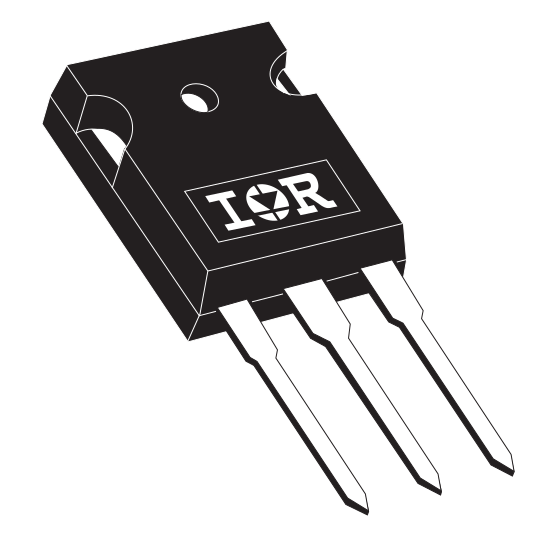
\includegraphics[scale=0.15]{Imagenes/IRFP150-TO247AC.png}
    \caption{MOSFET IRFP150N con su encapsulado THT de potencia tipo TO-247AC.}
    \label{irfp150}
\end{figure}

El encapsulado es del tipo TO-247AC, visible en la figura \ref{irfp150}. Este es un encapsulado through-hole o THT utilizado para dispositivos de alta disipación de potencia, por su tamaño y su superficie metálica que facilita la utilización de un disipador para mantener la temperatura bajo control.\\

\subsubsection{Selección de Diodos Rectificadores}

Ahora debemos seleccionar los cuatro diodos que conforman el rectificador de puente completo en el secundario del convertidor. Al igual que los transistores de la sección anterior, estos deben ser diodos de potencia capaces de manejar la potencia de \SI[]{300}[]{\watt} que circulará a través de ellos. Se enumeran a continuación los requerimientos que deben cumplir los diodos seleccionados:\\

\begin{itemize}
    \item Tensión inversa $V_R > \SI[]{150}[]{\volt}$.
    \item Corriente directa $I_F > \SI[]{4.5}[]{\ampere}$.
    \item Tiempo de recuperación de inversa $t_{rr}$ mucho menor al período de conmutación $T_s$ de \SI[]{50}[]{\micro\second}.
    \item Encapsulado THT capaz de manejar altas disipaciones de potencia.\\
\end{itemize}

Con estas especificaciones en cuenta, se eligieron los diodos ultrafast recovery de la serie MUR, particularmente el modelo MUR860 por su corto tiempo de recuperación inversa, baja caída de tensión en conducción y alta tensión inversa máxima. Se detallan sus especificaciones importantes en el siguiente cuadro.\\

\setlength{\tabcolsep}{7pt}
\renewcommand{\arraystretch}{1.5}
\begin{table}[h]
\begin{center}
    \begin{tabular}{llrrrr}
    {\SemiBold Fabricante} & {\SemiBold Modelo} & $\mathbf{V_{RRM}}$ [\unit{\volt}] & $\mathbf{I_{F(AV)}}$ [\unit{\ampere}] & $\mathbf{V_F}$ [\unit{\volt}] & $\mathbf{t_{rr}}$ [\unit{\nano\second}]\\
    \hline
    ON Semiconductor & MUR860 & \num{600} & \num{8} & \num{1.5} & \num{60}\\
    \end{tabular}
    \caption{Especificaciones del diodo rectificador ultrafast recovery MUR860 de ON Semiconductor.\textsuperscript{\cite{MUR860}}}
    \label{tabla:MUR860}
\end{center}
\end{table}

Donde $V_{RRM}$ es la máxima tensión inversa repetitiva, $I_{F(AV)}$ es la máxima corriente rectificada promedio, $V_F$ es la tensión directa instantánea y $t_{rr}$ el máximo tiempo de recuperación de inversa.\\

Estos son diodos rectificadores de potencia de la gama ultrafast recovery, pensados para aplicaciones en fuentes de corriente continua conmutadas, como es el caso de este convertidor. Como se ve en el cuadro \ref{tabla:MUR860}, este diodo tiene una tensión inversa máxima muy por encima de los requerimientos, al igual que la máxima corriente directa, que es cerca del doble de lo requerido, dando buenos márgenes de seguridad. Su tiempo de recuperación es similar a los tiempos de conmutación de los transistores IRFP150N de la tabla \ref{tabla:MUR860}, y su caída de tensión en directa de \SI[]{1.5}[]{\volt} es adecuadamente baja.\\

\begin{figure}[h]
    \centering
    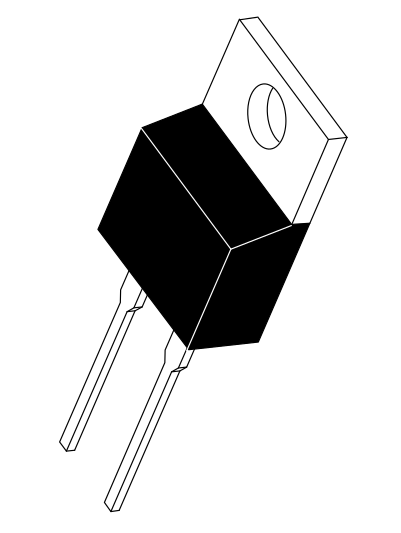
\includegraphics[scale=0.16]{Imagenes/MUR860.png}
    \caption{Diodo rectificador MUR860 con su encapsulado THT de potencia tipo TO-220AC.}
    \label{mur860}
\end{figure}

Se observa este diodo en su encapsulado THT de potencia tipo TO-220AC en la figura \ref{mur860}. Al igual que el encapsulado de los transistores IRFP150N, el TO-220AC posee una superficie metálica en contacto directo con el semiconductor interno que facilita la transferencia de calor hacia un disipador metálico.\\

\subsubsection{Transformador}

Habiendo seleccionado los transistores de potencia y rectificadores, corresponde ahora dimensionar el transformador que separa galvánicamente el puente de transistores del puente de diodos. Para todos los convertidores CC-CC conmutados y aislados, este transformador debe ser de alta frecuencia, que tiene algunas características particulares, necesarias reducir la inductancia parásita y las corrientes Eddy de pérdida en el núcleo, ya que estos parámetros se tornan más significativos a las altas frecuencias de conmutación de los convertidores.\\

La relación de vueltas $n$ del transformador de la figura \ref{puente_completo}, definida en este caso como la relación entre las vueltas del bobinado secundario $N_S$ y el bobinado primario $N_P$, viene dada por la siguiente ecuación, que resulta de calcular el cociente entre la tensión de secundario $V_S$ y la mínima tensión de primario $V_{P(min)}$.\textsuperscript{\cite{SoftSwitchPWM}\cite{StudyDesignFullBridge}}

\begin{equation}\label{relacion_vueltas}
    n = \frac{N_S}{N_P} = \frac{V_{S}}{V_{P(min)}} = \frac{(V_{out}+2V_F)\ /\ D_{sec(max)}}{V_{in(min)}-2V_{RDS(on)}}
\end{equation}

La tensión equivalente del secundario, en el numerador, viene dada por la suma de la tensión fija de salida $V_{out}$ de \SI[]{75}{\volt} y la caída de tensión en directa de los rectificadores $V_F$, que según la tabla \ref{tabla:MUR860} es de unos \SI[]{1.5}{\volt}, todo dividido por el ciclo de trabajo máximo en el secundario $D_{sec(max)}$, tomado en este caso como \num{0.8} u \num{80}\%.\\

Luego, en el denominador, se encuentra la expresión de la mínima posible tensión en el primario. Esta condición ocurre cuando la tensión que entrega la pila de combustible es la más baja en su curva V-I ($V_{in(min)}$), alrededor de \SI[]{28}{\volt}, coincidente con la máxima corriente de pila de \SI[]{10}{\ampere}. Luego, a esta tensión mínima se le resta la tensión de conducción $V_{RDS(on)}$ de ambos transistores que conforman un lazo con la pila y el bobinado primario, definida como la máxima caída de tensión sobre la resistencia drain-source de \SI[]{0.036}{\milli\ohm} detallada en la tabla \ref{tabla:IRFP150} para el transistor IRFP150.\\

Resumiendo, los datos para calcular el valor de la relación de vueltas en base a la ecuación anterior son los siguientes:

\begin{multicols}{2}
    \begin{itemize}
        \item $V_{out} = \SI[]{75}{\volt}$
        \item $V_F = \SI[]{1.5}{\volt}$
        \item $D_{sec(max)} = 0.8$
        \item $V_{in(min)} = \SI[]{28}{\volt}$
        \item $V_{RDS(on)} = \SI[]{10}{\ampere}\cdot\SI[]{0.036}{\ohm} = \SI[]{0.36}{\volt}$
        \item[\vspace{\fill}]       % Para que la segunda columna quede bien espaciada verticalmente con cantidad impar de elementos
    \end{itemize}
\end{multicols}

Con estos datos en cuenta, el valor necesario para la relación de vueltas del transformador de alta frecuencia del convertidor resulta:

\begin{equation}\label{relacion_vueltas_valor}
    \boxed{
    \highlight{\mathbf{n} = \frac{(V_{out}+2V_F)\ /\ D_{sec(max)}}{V_{in(min)}-2V_{RDS(on)}} = \num{3.57} \approx \num{3.6}}
    }
\end{equation}

\subsubsection{Filtro de Salida}

Con los diodos del rectificador de puente completo seleccionados, solo queda dimensionar el filtro LC de salida, compuesto por un inductor $L_f$ en serie y un capacitor $C_f$ en derivación (figura \ref{puente_completo}), que se encarga de transformar la onda rectificada a la salida del puente de diodos en una tensión continua para que se pueda conectar la plataforma al bus de continua del sistema híbrido.\\

Para poder asignarle valores a estos componentes, se deben definir dos parámetros de rendimiento del filtro: el ripple de corriente máximo del inductor $\Delta I_{L_f}$ en ampere, y el ripple de tensión pico a pico de salida $\Delta V_{out_{pp}}$. La selección de estos parámetros presenta una relación de compromiso, ya que a medida que se hacen más exigentes los requerimientos, genera valores de inductancia y capacidad más grandes. Esto resulta en componentes más grandes y difíciles de colocar en una PCB compacta cómo la que se busca obtener.\\

El ripple de corriente en el inductor viene dado por los ciclos de carga-descarga de $L_f$ : cuando la salida del rectificador es no nula, el inductor se carga con una pendiente fija; al conmutar a una tensión nula, se comienza a descargar a través de los diodos del rectificador, que actúan como rueda libre. Como el capacitor $C_f$ no puede tener una corriente continua (si fuese el caso, su tensión crecería sin límite), absorbe únicamente las variaciones de corriente con valor medio nulo, llegando a la carga únicamente la componente de corriente continua. El ripple de tensión que cae sobre la carga viene dado mayormente por la resistencia serie equivalente (ESR) del capacitor electrolítico.\textsuperscript{\cite{SoftSwitchPWM}}\\

Teniendo esto en cuenta, asignamos las siguientes cotas para el ripple de corriente de inductor y de tensión de salida:

\begin{itemize}
    \item $\Delta I_{L_f(max)} = \SI[]{0.8}{\ampere}$
    \begin{itemize}
        \item Es un ripple de corriente equivalente al 20\% de la máxima corriente de salida de \SI{4}{\ampere}.
    \end{itemize}
    \item $\Delta V_{out_{pp}(max)} = \SI[]{75}{\milli\volt}$
    \begin{itemize}
        \item Es un ripple de tensión equivalente al 0,1\% de la tensión fija de salida del bus de \SI[]{75}{\volt}.
    \end{itemize}
\end{itemize}

\paragraph{Cálculo del Inductor}

La ecuación \ref{ec_Lf} relaciona el valor de inductancia de salida $L_f$ con múltiples parámetros, de los cuales el más importante para nosotros es el ripple de corriente del inductor $\Delta I_{L_f(max)}$.\textsuperscript{\cite{SoftSwitchPWM}}

\begin{equation}\label{ec_Lf}
    L_f = \frac{V_{out}}{2f_s\cdot\Delta I_{L_f}}\left(1-\frac{V_{out}}{nV_{in(max)}-2V_F}\right)
\end{equation}

Dónde $V_{out}$ es la tensión continua de salida, de \SI[]{75}{\volt} en nuestro caso; $f_s$ es la frecuencia de conmutación en el primario, \SI[]{20}{\kilo\hertz} en esta plataforma; $\Delta I_{L_f}$ es el ripple ya mencionado; $n$ es la relación de vueltas del transformador, de valor \num{3.6} según la ecuación \ref{relacion_vueltas_valor}; $V_{in(max)}$ es la máxima tensión que entrega la pila, de unos \SI[]{45}{\volt} cómo se estableció al principio de la sección 3.2; y $V_F$ la caída de tensión en directa de los rectificadores, de \SI[]{1.5}{\volt} para los MUR860.\\ 

Reemplazando los valores en la ecuación, nos queda el siguiente valor para el inductor de filtro:

\begin{equation}\label{Lf_valor}
    \boxed{
    \highlight{\mathbf{L_f} = \frac{\SI{75}{\volt}}{2\cdot\SI{20}{\kilo\hertz}\cdot\SI{0.8}{\ampere}}\left(1-\frac{\SI{75}{\volt}}{\num{3.6}\cdot\SI{45}{\volt}-2\cdot\SI{1.5}{\volt}}\right) = \SI{1.24}{\milli\henry} \approx \SI{1.2}{\milli\henry}}
    }
\end{equation}

\paragraph{Cálculo del Capacitor}

Cómo se mencionó en la explicación del funcionamiento del filtro, la mayor parte del ripple de tensión, alrededor del 90\%, viene dado solo por la caída de tensión en la resistencia serie equivalente del capacitor electrolítico.\textsuperscript{\cite{SoftSwitchPWM}} El máximo valor de la resistencia serie equivalente viene dado por el cociente entre el ripple de tensión de salida y el ripple de corriente del inductor:

\begin{equation*}
    ESR_{max} = \frac{\Delta V_{out_{pp}(max)}}{\Delta I_{L_f(max)}} = \frac{\SI{75}{\milli\volt}}{\SI{0.8}{\ampere}} = \SI{93.75}{\milli\ohm}
\end{equation*}

Habiendo obtenido el máximo valor admisible de resistencia serie del capacitor, podemos usar la siguiente relación entre el valor de capacidad y ESR del capacitor.\textsuperscript{\cite{SoftSwitchPWM}}

\begin{equation}\label{Cf-ESR}
    C_f\cdot ESR = \num{60e-6}
\end{equation}

Despejando $C_f$ de la ecuación anterior, y utilizando el máximo valor admisible de resistencia serie equivalente que obtuvimos, podemos calcular el mínimo valor admisible de capacidad de filtro de salida para cumplir los requerimientos de ripple establecidos.

\begin{equation}\label{Cf_valor}
    \boxed{
    \highlight{\mathbf{C_{f(min)}} = \frac{\num{60e-6}}{ESR_{max}} = \frac{\num{60e-6}}{\SI{93.75}{\milli\ohm}} = \SI{640}{\micro\farad}}
    }
\end{equation}

Ahora, solo queda la selección de algún modelo comercial de capacitor electrolítico de valor nominal mayor a la cota mínima establecida por la ecuación anterior. Como en el secundario pueden llegar a existir tensiones transitorias muy elevadas que superan los \SI{100}{\volt} (esto sin tener en cuenta los posibles sobrepicos de tensión en el sistema real), se debe seleccionar un capacitor electrolítico con un nivel de tensión elevado.\\

\begin{figure}[h]
    \centering
    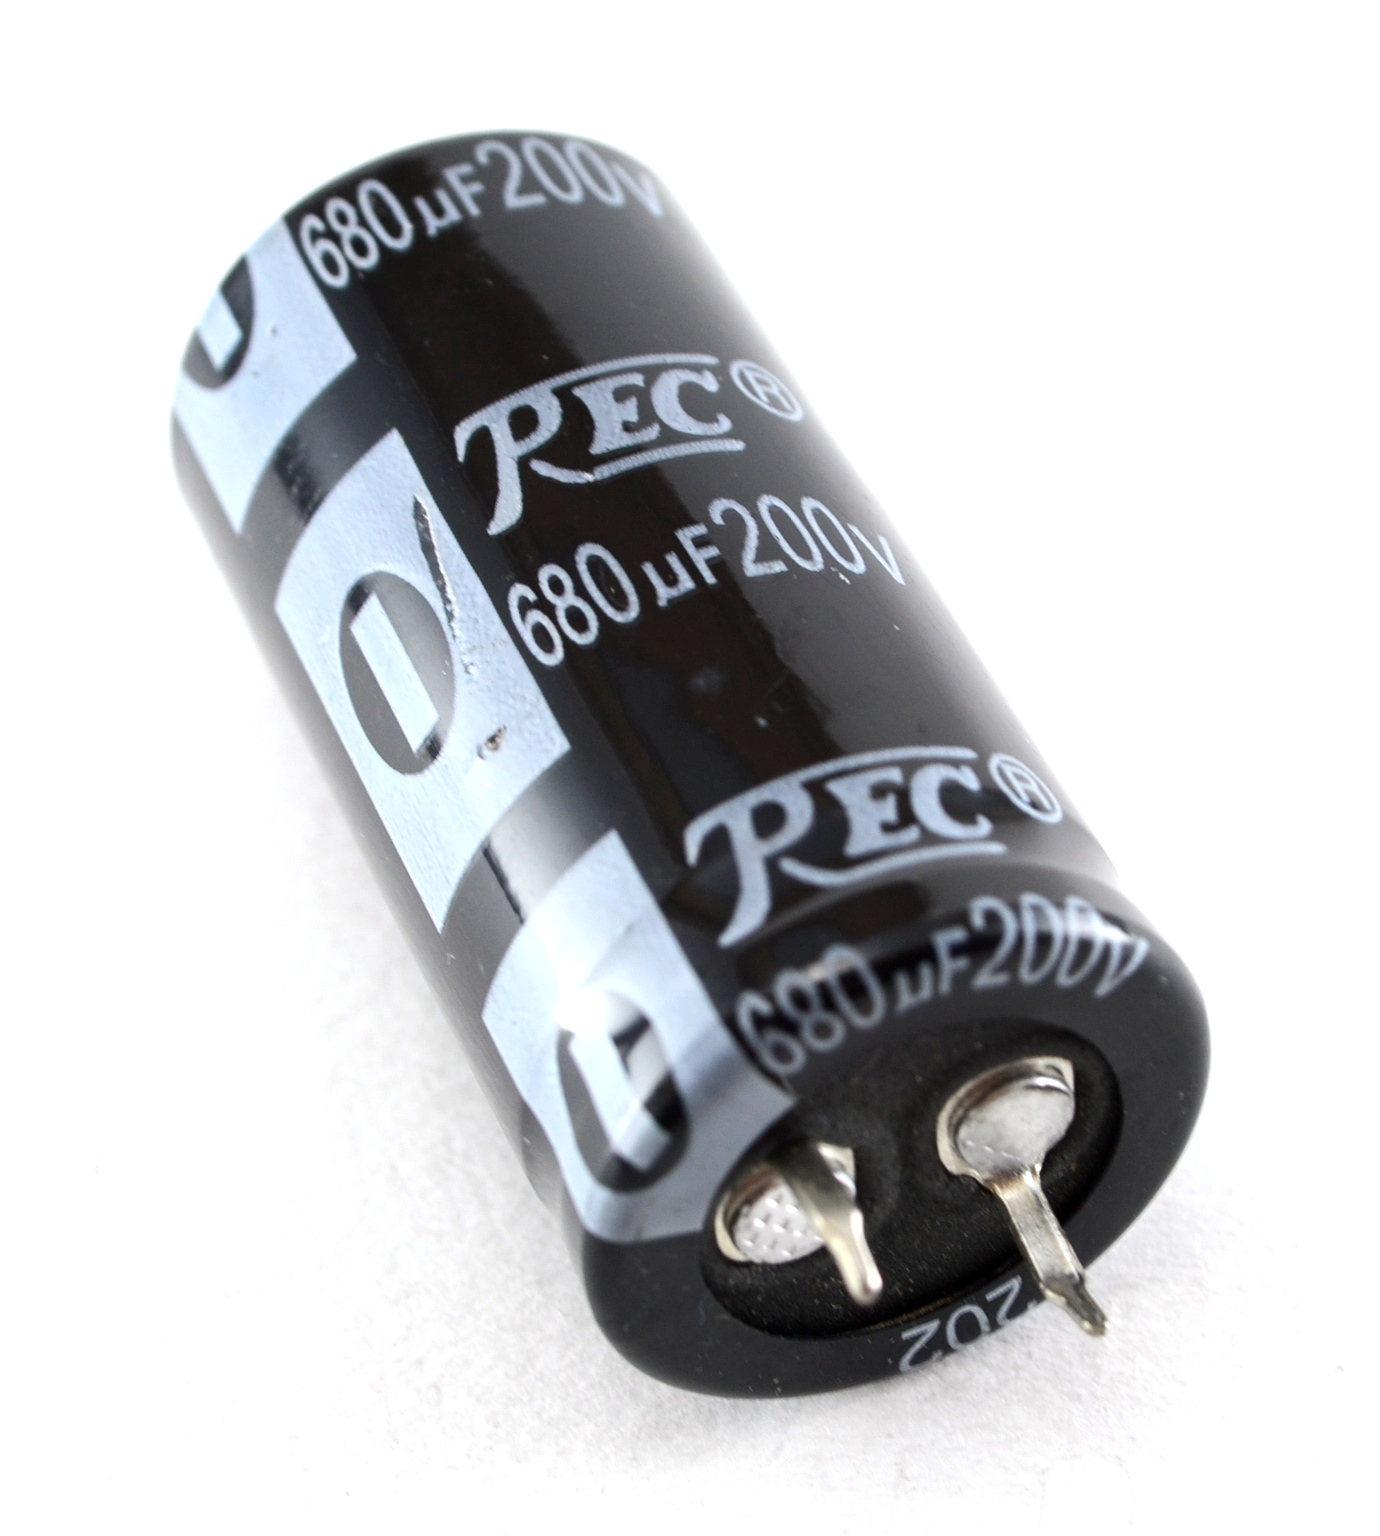
\includegraphics[scale=0.20]{Imagenes/Capacitor Blindado.jpg}
    \caption{Capacitor electrolítico blindado de \SI{680}{\micro\farad} y \SI{200}{\volt}, similar al utilizado en la plataforma.}
    \label{Cf_blindado}
\end{figure}

En base a disponibilidad de proveedores locales de componentes eléctricos, se seleccionó un capacitor electrolítico blindado de \SI{200}{\volt} de tensión, y de un valor de capacidad de \SI{680}{\micro\farad}, que es el valor de capacidad comercial superior al resultado de \ref{Cf_valor} más cercano a la cota. Se puede observar en la figura \ref{Cf_blindado} un modelo similar al que se utilizó en la placa.\\